% Autor: Martin Hofbauer, Brno 2022
% ###########################################################################
\chapter{Úvod}
% ###########################################################################
TODO

\chapter{Výběr technologií}
TODO
\section{Programovací jazyk}
Jednou z nejdůležitějších částí při výběru použitých technologií je právě programovací jazyk. V našem případě je nutné zvolit takový, ve kterém aplikace poběží velmi rychle. Také je důležité (https://link.springer.com/article/10.1186/1471-2105-9-82)

\section{Meziprocesní komunikace}
TODO(k čemu)
\subsection{Roury}
\subsection{TCP/IP}
TODO(co jsem vybral)



% ###########################################################################
\chapter{Návrh systému}
% ###########################################################################
TODO

% ###########################################################################
\chapter{Implementace}
% ###########################################################################
TODO
\begin{figure}[hbt]
	\centering
	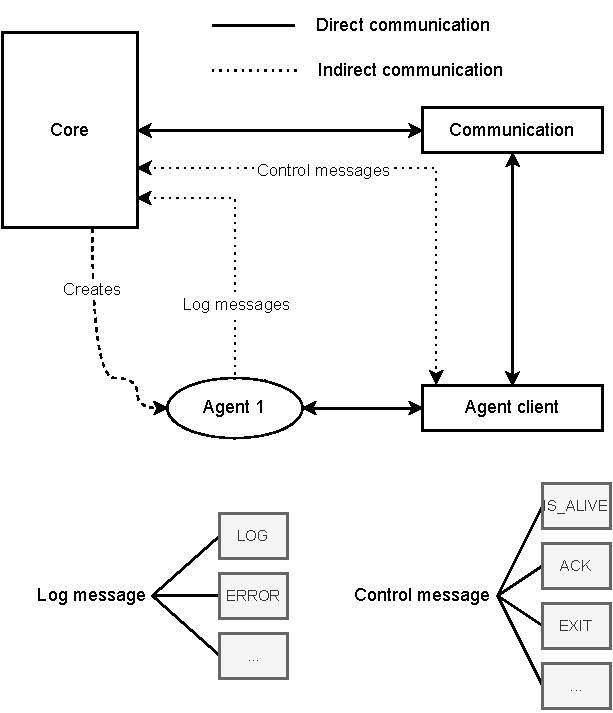
\includegraphics[width=\textwidth]{diagrams/architecture/architecture_diagram.pdf}
	\caption{Architektura systému}
\end{figure}
\begin{figure}[hbt]
	\centering
	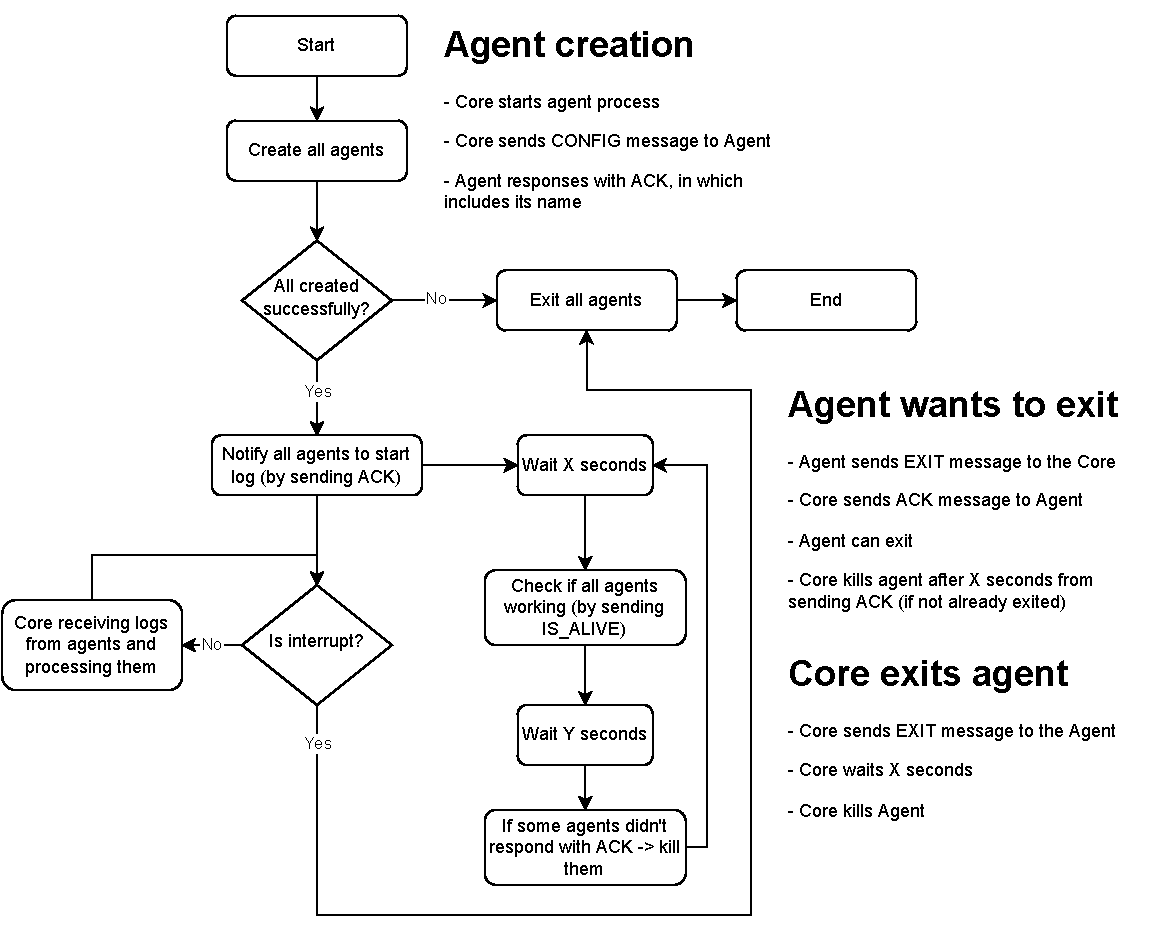
\includegraphics[width=\textwidth]{diagrams/flowchart/flowchart.pdf}
	\caption{Vývojový diagram chování systému}
\end{figure}
\begin{figure}[hbt]
	\centering
	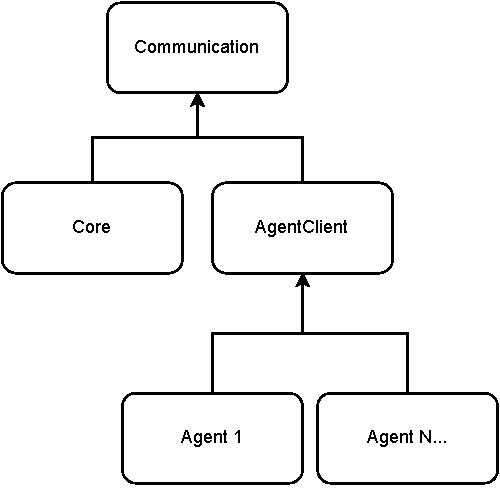
\includegraphics[width=\textwidth]{diagrams/dependency-diagram/dependency_diagram.pdf}
	\caption{Diagram závislostí}
\end{figure}

% ###########################################################################
\chapter{Testování}
% ###########################################################################
TODO

% ###########################################################################
\chapter{Závěr}
% ###########################################################################
TODO



